\documentclass[14pt]{article}
\usepackage{listings}
\usepackage{color}
\usepackage{graphicx}
\usepackage{setspace}

\definecolor{dkgreen}{rgb}{0,0.6,0}
\definecolor{gray}{rgb}{0.5,0.5,0.5}
\definecolor{mauve}{rgb}{0.58,0,0.82}

\lstset{frame=tb,
  language=java,
  aboveskip=3mm,
  belowskip=3mm,
  showstringspaces=false,
  columns=flexible,
  basicstyle={\small\ttfamily},
  numbers=none,
  numberstyle=\tiny\color{gray},
  keywordstyle=\color{blue},
  commentstyle=\color{dkgreen},
  stringstyle=\color{mauve},
  breaklines=true,
  breakatwhitespace=true
  tabsize=3
}







\begin{document}
\title{% 
  \huge Concurrent and Distributed Systems \\
  \vspace{20mm}
  \large Laboratory Assignment \\}

\date{\today}
\maketitle
\begin{center}
\vspace{30 mm}

\title{\huge Student: Marcu Andrei Cristian}
\\\vspace{10 mm}
\title{\huge Computers and Information Technology}
\\\vspace{10 mm}
\title{\huge CEN 3.2 A}
\\\vspace{10 mm}
\title{\huge 3rd Year}
\end{center}
\date{}
\maketitle

\newpage
\section*{Problems statements}
\vspace{20 mm}
\textbf{Problem 1} (50p) \\
Find all prime numbers in [1,n] using k threads. Let n =
kq + r, where 0 ≤ r <k where r is the remainder of n divided to k. You should
consider 2 solutions:\\
- Partition the interval [1,n] in k intervals as follows: I1=[1,q+1], I2=[q+2,
2q+2], . . . , Ir=[(r-1)q+r, rq+r], Ir+1=[rq+r+1, (r+1)q+r], ..., Ik=[(k-1)q+r+1,
kq+r]. Each thread 1 ≤ j ≤ k will determine the prime numbers in the Interval
Ij .\\
- The multiples of k+1 strictly bigger than k+1 are not prime numbers. These
numbers should be eliminated from the interval [1,n] resulting in set M. This
set should be partitioned in k subsets as follows: for each 1 ≤ j ≤ k the set Mj
contains all those elements from M who by divided with k+1 give remainder j.
Also it is considered that k+1 belongs to M1. Each thread j will determine the
prime numbers from set Mj .\\
Which of the solutions is better and why?
\\\vspace{10 mm}\\
\textbf{Problem 2} (50p) \\
What values can n have at the end of the concurrent counting algorithm execution?
\\
Assignment: Implement this algorithm in Java. What values do you get at the
end for n? \\
Assignment: Prove the above by describing in the technical reports a few test
scenarios and different states as shown in the first course.\\
\begin{center}
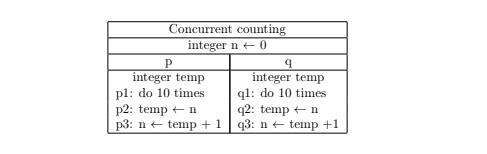
\includegraphics[height=1.8in, width = 5in]{problem2.png}\\
\end{center}
\newpage
\\\vspace{10 mm}\\
\textbf{Problem1:} As we've seen in the statement we need to find all the prime numbers in the [1,n] interval using k threads. Each thread should iterate through a smaller interval which can be defined using the generalised formula Ik = [(k-1)q + r + 1, kq + r]. The formula will skip the numbers from [1, r] so we need to treat that separately.
\\\vspace{1 mm}\\
For example for an input like this: n = 10 k = 2.\\
The prime numbers in the [1,n] interval are : 2, 3, 5, 7\\
q = 10/2 = 5 ; r = 10 \% 2 = 0 . Because r is 0 we don't need to check the ones from [1,r] \\
We've got k = 2 so 2 threads.\\
T1 = [(1 - 1) * 5 + 0 + 1, 1 * 5 + 0] = [1, 5]\\
T2 = [(2 - 1) * 5 + 0 + 1, 2 * 5 + 0] = [6, 10]\\
Each of those threads will iterate through the smaller intervals presented before.
\\\vspace{1 mm}\\
For example for an input like this case: n = 8 k = 3.\\
The prime numbers in the [1,n] interval are : 2, 3, 5, 7\\
q = 10/2 = 2 ; r = 10 \% 2 =2 . Because r is 2 we need to check the ones from [1,r] \\
We've got k = 3 so 3 threads.\\
T1 = [(1 - 1) * 2 + 2 + 1, 1 * 2 + 2] = [3, 4]\\
T2 = [(2 - 1) * 2 + 2 + 1, 2 * 2 + 2] = [5, 6]\\
T3 = [(3 - 1) * 2 + 2 + 1, 3 * 2 + 2] = [7, 8]\\
So the numbers from 1 to r ( 1 to 2) will not be checked. I've treated this case separately. Thread number 1 will check those numbers\\
Each of those threads will iterate through the smaller intervals presented before.
\\\vspace{1 mm}\\
\textbf{Problem2:} As we've seen in the statement we have 2 threads incrementing the same variable n 10 times. N is a global variable(static in my solution) so it will have the same value for all instances of the ConcurrentThread class.\\
For example the result for the input presented in the solution ( 2 threads, 10 iterations each) n will always reach the value 20.\\
I'll explain more examples later on my presentation.\\
Now that we've clarified the Problems Statements we can move on to the implementation.
\newpage

\section*{Solution Problem 1}\\
\textbf{Method1}\\
\begin{lstlisting}
//----------------------------PrimeThreadMethod1.java----------------------------
import java.util.ArrayList;
import java.util.Collections;
import java.util.List;

public class PrimeThreadMethod1 extends Thread{
	private int threadNumber; // thread it
	private int n, k, q, r;
	
	public static volatile List<Integer> primeNumbers = Collections.synchronizedList (new ArrayList<Integer>());
	// In this list we add prime numbers everytime we find one.
	//It's a synchronizedList in order to be thread-safe.
	PrimeThreadMethod1(int n, int k, int threadNumber)
	{
		this.n = n;
		this.k = k;
		this.threadNumber = threadNumber;
		this.q = this.n / this.k;
		this.r = n % k;
		
		if(k > n)
			throw new ArrayIndexOutOfBoundsException("More threads than numbers"); 
		// We can't have more threads than numbers.
	}
	public void run()
	{
		//The general formula doesn't treat the case from [1, r]. So i've added the numbers from [1, r] to thread number 1.
		int rest;
		if(threadNumber == 1)
			rest = 0;
		else
			rest = r;
		for( int i = (threadNumber - 1) * q + rest + 1; i <= threadNumber * q + r; i++)	
			//We split the interval in multiple invervals using the threadNumber
		{
			Boolean primeFlag = false;
			//Boolean value that checks if the number is prime or not
			int sqrt = (int) (Math.ceil(Math.sqrt((double) i )));
			// sqrt in order to iterate from 2 to sqrt
			for( int j = 2 ; j <= sqrt; j++ )
			{
				if( i == 2 )// 2 is the first prime number
				{
					//System.out.println("Thread number " + threadNumber + " added the number :" + i);
					primeFlag = true;
					primeNumbers.add(i);
					// we add 2 in the ArrayList, we make the flag true so we don't add 2 two times, and we break the loop because the next values are pointless.
					break;
				}
				if(i % j == 0)
				{
					primeFlag = true;
					//we've found a divider, the number is not prime. We break the loop because the next values are pointless.
					break;
				}
			}
			if(primeFlag == false && i != 1)
			{
				//System.out.println("Thread number " + threadNumber + " added the number :" + i);
				primeNumbers.add(i);
				//If the number it's not prime and it is different than 1 we add it in the ArrayList.
			}
		}
	}
}

\end{lstlisting}
\vspace{5 mm}\\
\textbf{Method2}\\
\begin{lstlisting}
//----------------------------PrimeThreadMethod2.java----------------------------
import java.util.ArrayList;
import java.util.Collections;
import java.util.List;
import java.util.Map.Entry;
import java.util.concurrent.ConcurrentHashMap;

public class PrimeThreadMethod2 extends Thread{
	private int threadNumber; // Thread identifier
	
	public static volatile ConcurrentHashMap<Integer, ArrayList<Integer> > splitedInterval = new ConcurrentHashMap<Integer, ArrayList<Integer>>(); 
	// I've used a map which keeps the numbers each thread should check
	// So each splitedInterval[threadId] will have an arrayList which contains the numbers it should check.
	// This map is created in main. If we create it inside the class the code will be executed multiple times.
	// I've used ConcurrentHashMap in order to be thread safe.
	public static volatile List<Integer> primeNumbers = Collections.synchronizedList (new ArrayList<Integer>());
	// The list contains the prime numbers we find. It's a synchronizedList which is thread-safe.
	PrimeThreadMethod2(int n, int k, int threadNumber)
	{
		this.threadNumber = threadNumber;		
		if(k > n)
			throw new ArrayIndexOutOfBoundsException("More threads than numbers"); 
		// We can't have more threads than numbers
	}
	public void run()
	{
		for( Entry<Integer, ArrayList<Integer>> entry: PrimeThreadMethod2.splitedInterval.entrySet()) 
			// We iterate through all the elements in map
	    {
	    	if(threadNumber - 1 == entry.getKey()) 
	    		// We check if we found the key which is equal to threadId
	    	{
	    		for(int i: entry.getValue()) 
	    			// We get the arrayList which has the key equal to threadId
	    		{
					Boolean primeFlag = false; 
					//Boolean value that checks if the number is prime or not
					int sqrt = (int) (Math.ceil(Math.sqrt((double) i )));
					// sqrt in order to iterate from 2 to sqrt
					for( int j = 2 ; j <= sqrt; j++ )
					{
						if( i == 2 )
							// 2 is the first prime number
						{
							//System.out.println("Thread number " + threadNumber + " added the number :" + i);
							primeFlag = true;
							primeNumbers.add(i);
							// we add 2 in the ArrayList, we make the flag true so we don't add 2 two times, and we break the loop because the next values are pointless.
							break;
						}
						if(i % j == 0)
						{
							primeFlag = true;
							//we've found a divider, the number is not prime. We break the loop because the next values are pointless.
							break;
						}
					}
					if(primeFlag == false && i != 1)
					{
						//System.out.println("Thread number " + threadNumber + " added the number :" + i);
						primeNumbers.add(i);
						//If the number it's not prime and it is different than 1 we add it in the ArrayList.
					}
	    		}
	    	}
		}	
	}
}

\end{lstlisting}
\vspace{5 mm}\\
\textbf{Main}\\
\begin{lstlisting}
//----------------------------MainThread.java----------------------------
import java.io.FileNotFoundException;
import java.io.PrintWriter;
import java.io.UnsupportedEncodingException;
import java.util.ArrayList;
import java.util.Random; 

public class MainThread {

	public static void main(String[] args) throws FileNotFoundException, UnsupportedEncodingException {
		PrintWriter writer = new PrintWriter("execution-output.txt", "UTF-8"); // writer used to print in file
		Random rand = new Random(); 
		// random instance
		int n = rand.nextInt(2000000);
		// random int from 1 to 2000000
	    //int k = rand.nextInt(2000000);
	    //int n = 37028;
	    int k = 2000;

	    while(k > n)
	    {
	    	k = rand.nextInt(2000); 
	    	// we make sure that we don't have more threads than numbers
	    }    

	    long startTime = System.currentTimeMillis(); 
	    // the time when we start the threads
	    
	    PrimeThreadMethod1[] t = new PrimeThreadMethod1[k];
	    for(int i = 1; i <= k; i++ ){
	       t[i-1] = new PrimeThreadMethod1(n, k, i);
	       //We create k threads and start them
	       t[i-1].start();
	    }
	    //We wait for the threads to finish
	    for(int i = 0; i < k; i++ ){
	       try {
	           t[i].join();
	       } catch (InterruptedException e) {
	           e.printStackTrace();
	       }
	    }
	    //the time when we finish
	    long stopTime = System.currentTimeMillis();
	    //the time of execution
	    long elapsedTime = stopTime - startTime;
	    
	    //We print the result in file
	    writer.println("#####################Method1#####################");
	    writer.println("Numbers from 1 to " + n);
	    writer.println("Number of threads is " + k);
	    writer.println("Execution time : " + elapsedTime/1000 + "," + elapsedTime%1000 + "s");
	    writer.println("All the prime numbers:" + PrimeThreadMethod1.primeNumbers.toString());
	    //Random lines to separate the methods
	    writer.println("###########################################################################");
	    writer.println("###########################################################################");
	    writer.println("###########################################################################");
	    writer.println("###########################################################################");
	    writer.println("###########################################################################");
	    
	    for(int i = 1; i <= n; i++)
	    	// We create the splittedInterval map
	    {
	    	if(i % (k+1) == 0 && i > (k + 1))
	    	{
	    		continue; 
	    		// If i is divided by (k+1) without rest and it is bigger than (k+1) it can't be prime number
	    	}
	    	if(!PrimeThreadMethod2.splitedInterval.containsKey(i % (k+1)))
	    		// The key will be the threadId
	    	{
	    		PrimeThreadMethod2.splitedInterval.put(i % (k+1), new ArrayList<Integer>());
	    		//We check if we already created the key in the map. If not we create it
	    	}
	    	if(i % (k + 1) == k) {
	    		PrimeThreadMethod2.splitedInterval.get(1).add(i);
	    		// My threads are from 0 to k - 1. The operation % (k + 1) will generate results from 0 to k.
	    		// So if the result is k we move that value to thread 1.
	    		continue;
	    	}
	    	//We add the value in the arrayList
	    	PrimeThreadMethod2.splitedInterval.get(i % (k+1)).add(i);
	    }
	    
	    
	    startTime = System.currentTimeMillis(); 
	    // the time when we start the threads
	    
	    PrimeThreadMethod2[] t2 = new PrimeThreadMethod2[k];
	    for(int i = 1; i <= k; i++ ){
	       t2[i-1] = new PrimeThreadMethod2(n, k, i);
	       //We create k threads and start them
	       t2[i-1].start();
	    }
	    //We wait for the threads to finish
	    for(int i = 0; i < k; i++ ){
	       try {
	           t2[i].join();
	       } catch (InterruptedException e) {
	           e.printStackTrace();
	       }
	    }
	    //the time when we finish
	    stopTime = System.currentTimeMillis();
	    elapsedTime = stopTime - startTime;
	    //the time of execution
	    
	    //We print the result in file
	    writer.println("#####################Method2#####################");
	    writer.println("All the prime numbers:" + PrimeThreadMethod2.primeNumbers.toString());
	    writer.println("Numbers from 1 to " + n);
	    writer.println("Number of threads is " + k);
	    writer.println("Execution time : " + elapsedTime/1000 + "," + elapsedTime%1000 + "s");
	    
	    System.out.println("Check output file"); 
	    // Console warning that tells us the results are in folder.
	    writer.close(); 
	    // We close the file writer.
	}
}

\end{lstlisting}
\section*{Experiments and results for problem 1}
\\\\\\
\begin{center}
1. Example with n = 50, k = 20.
\vspace{10mm}

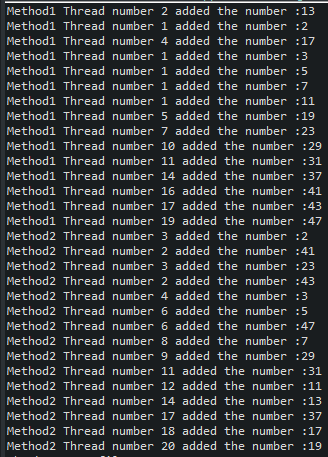
\includegraphics[height=4.5in, width = 5in]{5020thread.png}\\
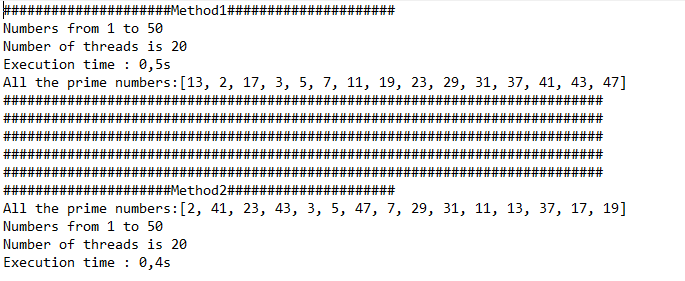
\includegraphics[height=3.5in, width = 6in]{5020result.png}\\
\newpage
\end{center}\\


\newpage

\begin{center}
2. Example with n = 500, k = 60.
\vspace{10mm}

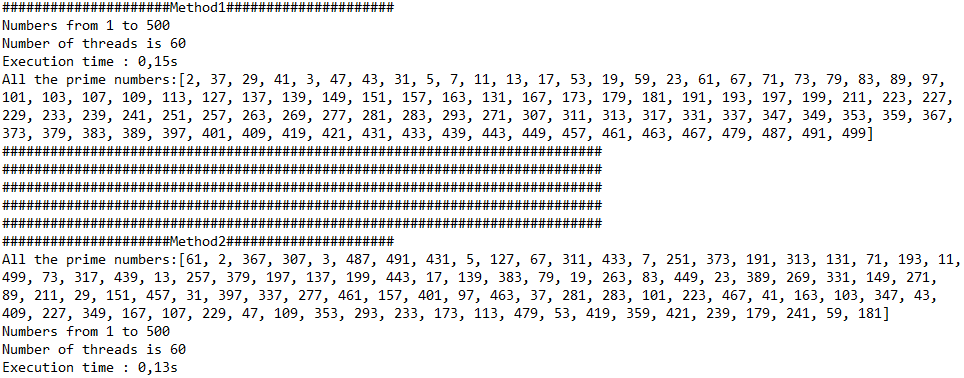
\includegraphics[height=5.5in, width = 6in]{50060result.png}\\
\end{center}\\
For bigger examples I can't print which thread adds the number because the result is too big.


\newpage

\begin{center}
3. Example with n = 3000, k = 200.
\vspace{10mm}

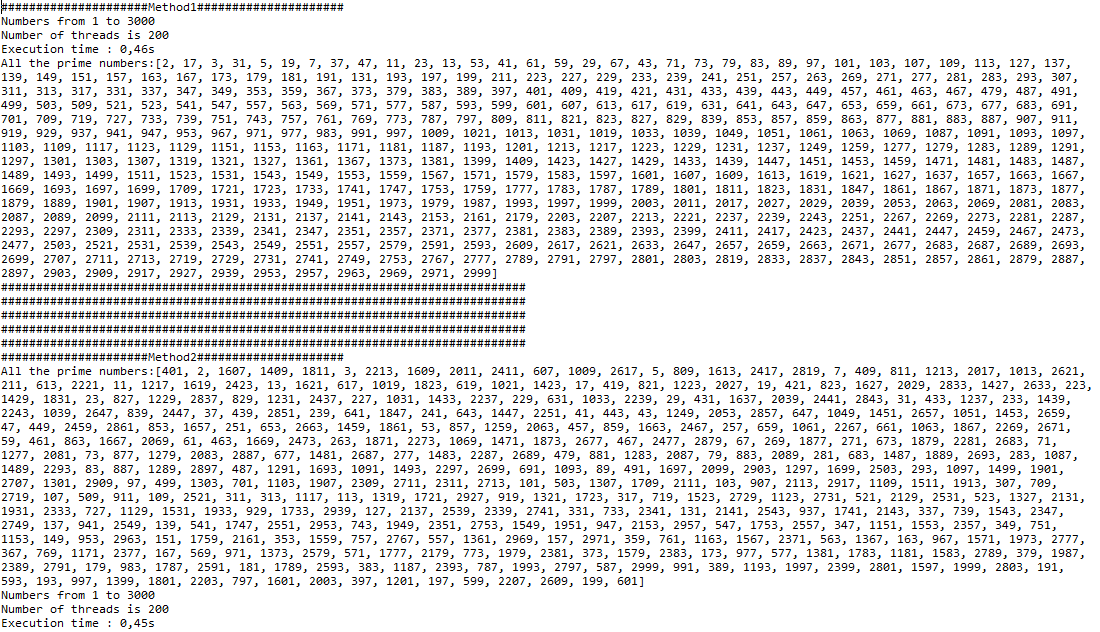
\includegraphics[height=5.5in, width = 6in]{3000200.png}\\
\end{center}\\
For bigger examples I can't print which thread adds the number because the result is too big.\\
Random generated bigger examples will be found in the txt files from the Experimental data and results directory.


\section*{Conclusions Problem 1}
\vspace{10 mm}
Working on this problem, I have acquired lots of knowledge about thread programming, data containers which are thread-safe and the problems normal data containers can cause. Both methods are equal if we talk about the execution time, sometimes the first method finished faster, sometimes the second one.  
\newpage

\section*{Solution Problem 2}\\
\textbf{Thread Class}\\
\begin{lstlisting}
//----------------------------ConcurrentThreadMethod1.java----------------------------

public class ConcurrentThread extends Thread {
	static volatile int n = 0; // I've used static in order to keep it's value in all the instances of ConcurrentThread class. 
	//Also it is a volatile variable because the cache memory of each thread can alter the value, so using volatile will make it thread-safe, the value being saved in memory instead of CPU cache.
	String message;// To keep an identification for threads.
	private int temp;
	
	public ConcurrentThread(String message)
	{
		this.message = message; // thread id
		this.temp = 0; // temp value is initially 0
	}
	
	public void run() {
		for(int i = 1 ; i <= 10; i++)
		{
			this.temp = n;
			n = this.temp + 1;
			System.out.println("The value of n in " + this.message + " iteration " + i + " is " + n);
		}
	}
}


\end{lstlisting}

\vspace{5 mm}\\
\textbf{Main}\\
\begin{lstlisting}
//----------------------------MainThread.java----------------------------

public class MainThread {

	public static void main(String[] args) {
		//We create 2 threads
		ConcurrentThread Thread1 = new ConcurrentThread("Thread1");    
        ConcurrentThread Thread2 = new ConcurrentThread("Thread2");
        //We start both threads
        Thread1.start();
        Thread2.start();
        //We wait until threads finish
        try {
        	Thread1.join();
        	Thread2.join();
        }
        catch(InterruptedException e){
        	e.printStackTrace();
        }
        //We print the value of n
        
        System.out.println("Last n value : " + ConcurrentThread.n);
	}

}


\end{lstlisting}
\section*{Experiments and results for problem 2}
\\\\\\
\begin{center}
1. Example with 10 iterations.
\vspace{10mm}

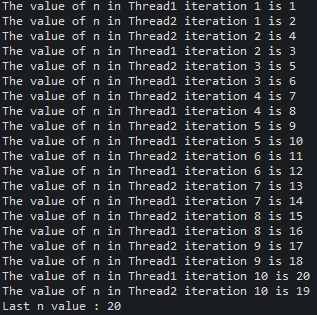
\includegraphics[height=3.5in, width = 5in]{problem220.png}\\
\end{center}\\
\newpage
\begin{center}
2. Example with 1000 iterations.
\vspace{10mm}

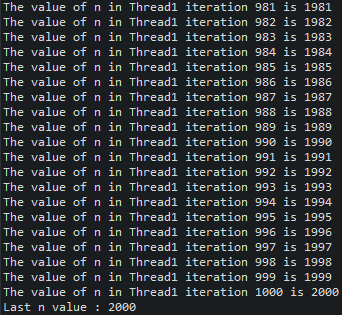
\includegraphics[height=3.5in, width = 5in]{problem22000.png}\\
\end{center}\\
\newpage

\begin{center}
3. Example with 1000000 iterations.
\vspace{10mm}

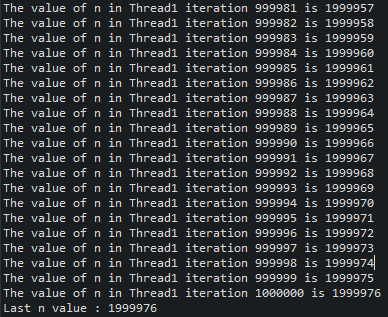
\includegraphics[height=3.5in, width = 5in]{problem21000.png}\\
\end{center}\\
Bigger examples will be found in the txt files from the Experimental data and results directory.
\newpage


\section*{Conclusions Problem 2}
\vspace{10 mm}
The conclusion of the examples presented before is that n should be 2 * number of iterations. Even though when we've got a big number of iterations n won't finish with the value we expect. This happens because of the memory synchronization. Even if we use volatile variable it will still have the same value. Thread race conditions can make the increment operation to be missed. In order to prevent this problem we should use an AtomicInteger which is thread-safe. If we use "synchronize" only one thread can modify the variable at a time and the problem would be solved.

\newpage
\section*{References}
\large https://en.wikipedia.org/wiki/Race_condition#Software
\\
\\\vspace{6mm}
\\
https://stackoverflow.com/questions/14983847/make-multiple-threads-use-and-change-the-same-variable
\\
\\\vspace{6mm}
\\
https://docs.oracle.com/javase/8/docs/api/java/util/concurrent/ConcurrentHashMap.html
\\
\\\vspace{6mm}
\\
https://www.geeksforgeeks.org/collections-synchronizedlist-method-in-java-with-examples/
\\
\\\vspace{6mm}
\\
https://www.geeksforgeeks.org/synchronized-in-java/

\end{document}